\documentclass[a4paper]{article}
\usepackage[14pt]{extsizes}
\usepackage[T2A]{fontenc}
\usepackage[utf8]{inputenc}
\usepackage[russian]{babel}
\usepackage{setspace,amsmath}
\usepackage{graphicx}
\usepackage{epigraph} 
\usepackage{csquotes} 
\usepackage[unicode, pdftex]{hyperref} 
\usepackage{amssymb} 
\usepackage{caption}
\usepackage{amsthm} 
\usepackage{wrapfig}
\usepackage[left=15mm, top=10mm, right=10mm, bottom=15mm, nohead, footskip=10mm]{geometry} 
\RequirePackage{caption}
\DeclareCaptionLabelSeparator{d}{}
\captionsetup{justification=centering,labelsep=d}

\begin{document}
\title{\textbf{Лабораторная работа 1.4.1}

\

Изучение экспериментальных погрешностей на примере физического маятника.

\
}
\author{И. М. Артёмов}
\date{7 октября 2022 г.}
\maketitle
\noindent
\textbf{Цель работы}: 1) на примере измерения периода свободных колебаний физического маятника познакомиться с систематическими и случайными погрешностями, прямыми и косвенными измерениями; 2) проверить справедливость формулы для периода колебаний физического маятника и определить значение ускорения свободного падения; 3) убедиться в справедливости теоремы Гюйгенса об обратимости точек опоры и центра качания маятника; 4) оценить погрешность прямых и косвенных измерений и конечного результата.

\

\noindent
\textbf{Оборудование}: 	металлический стержень с опорной призмой; закреплённая на стене консоль; подставка с острой гранью для определения центра масс маятника; секундомер; счётчик колебаний (механический или электронный); линейки металлические различной длины; штангенциркуль; электронные весы; математический маятник (небольшой груз, подвешенный на нитях).

\section*{\textbf{1. Теоретическое введение.}}

Пусть однородный стержень длины $l$ подвешен на оси $O$ на расстоянии $a$ от центра масс $C$. При отклонении стержня от вертикали на угол $\varphi \ll 1$, начинаются колебания стержня, которые можно описать уравнением моментов относительно оси $O$:
\begin{equation}
I \ddot{\varphi} \approx - m g a \varphi,
\end{equation}

\noindent
где $\varphi$ - угол отклонения маятника от вертикали, $m$ - его масса, $I$ - момент инерции относительно оси подвеса.

\noindent
Имеем дело с уравнением гармонических колебаний с периодом:
\begin{equation}
T = 2\pi \sqrt{\frac{I}{mga}}
\end{equation}

\noindent
С учётом теоремы Гюйгенса-Штейнера: $I = \frac{ml^2}{12} + m a^2$, получим:
\begin{equation}\label{eq3}
T = 2\pi \sqrt{\frac{\frac{l^2}{12} + a^2}{g a}}
\end{equation}

\noindent
Заметим, что если положить:
\begin{equation}
l_{\text{пр}} = \frac{l^2}{12 a} + a,
\end{equation}
получим, что период равен периоду колебаний математического маятника с длиной $l_{\text{пр}}$.




\begin{flalign*} \text{Заметим, что  } \frac{dl_{\text{пр}}}{da} = 1 - \frac{l^2}{12 a^2} \text{ , отсюда } a_{m} = \frac{l}{2\sqrt{3}} \text{ --- значение $a$, при котором период} \end{flalign*} $T$ минимален.

\noindent
Докажем также \textit{теорему Гюйгенса}. Пусть период одинаков при $a=a_1$ и $a=a_2$. Тогда:
\[\forall a\in \{a_1, a_2 \} \hookrightarrow a + \frac{l^2}{12 a} = l_\text{пр}(a_1) \Rightarrow a^2 - l_\text{пр}(a_1) a + \frac{l^2}{12} = 0 \Rightarrow \]
\[\Rightarrow a_1 + a_2 = l_\text{пр}(a_1), \]
то есть если сместить точку подвеса на расстояние $l_\text{пр}$ вниз,
то период колебаний не изменится.

\begin{figure}
\begin{minipage}{0.49\linewidth}
\center{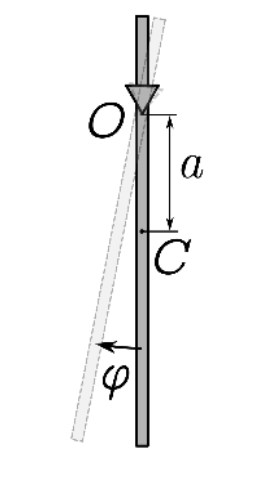
\includegraphics[scale=0.5]{pictures/рис 1.png}}
\caption{.\ \textit{Стержень как физический маятник}}
\end{minipage}
\hfill
\begin{minipage}{0.49\linewidth}
\center{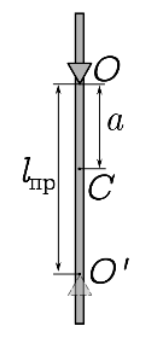
\includegraphics[scale=0.7]{pictures/рис 2.png}}
\caption{.\ \textit{К теореме Гюйгенса}}
\end{minipage}
\end{figure}

\noindent
В работе также будет изучаться затухание колебаний. Предполагая, что диссипация обусловлена вязким трением, пропорциональным угловой скорости маятника, получим для мощности потерь:
\begin{equation}
P = -\alpha \dot{\varphi}^2 \quad (\alpha > 0),
\end{equation}
Усредним $P$ по периоду, считая затухание малым:
\[\langle P \rangle_T = \langle -\xi E_\text{к}(t) \rangle_T \approx -\xi \frac{E}{2} \quad (\xi > 0),\] 
где $E$ - энергия системы в данном периоде. То есть:
\[\frac{dE}{dt} = -\xi \frac{E}{2}, \text{ откуда: } E = E_0 \exp{(-2 \gamma t)} \quad (\gamma = \xi/4) \Rightarrow \]

\noindent
\begin{equation}
\Rightarrow A(t)= A_0 \exp{(-\gamma t)} 
\end{equation}

\noindent
За время $\tau = 1/\gamma$ амплитуда $A$ колебаний падает в $e$ раз. Отношение времени жизни колебаний к периоду определяет добротность системы:
\begin{equation}
Q = \pi \frac{\tau}{T}
\end{equation}
Параметр $\tau$ легко определить, зная время $\tau_2$, за которое амплитуда падает в $2$ раза:
\begin{equation}
\tau = \frac{\tau_2}{\ln 2}
\end{equation}
Наконец, добавим поправки к формуле \eqref{eq3}, учитывающие, конечные массу и размер призмы. Точная формула имеет вид:
\begin{equation}
T = 2\pi \sqrt{\frac{I_{\text{ст}} + I_{\text{пр}}}{m_{\text{ст}} g a - m_{\text{пр}} g a_{\text{пр}}} }
\end{equation}

\noindent
Здесь $I_{\text{пр}}, m_{\text{пр}}, a_{\text{пр}}$ - соответственно момент инерции призмы относительно оси подвеса, её масса и расстояние от оси подвеса до центра масс призмы (знак "минус" в знаменателе означает, что призма находится над осью).

\noindent
Заметим, что $m_{\text{пр}} \sim 10^{-1} \text{ кг}$, $a_{\text{пр}} \sim 1 \text{ см}$, $m_{\text{ст}} \sim 1 \text{ кг} $, $a \geq 10 \text{ см}$, поэтому $I_{\text{пр}}/I{\text{ст}} \sim 10^{-3}$. Это означает, что можно не учитывать $I_{\text{пр}}$. Однако для моментов, создаваемых силами тяжести призмы и стержня, имеем:
\[\frac{M_{\text{пр}}}{M_{\text{ст}}} = \frac{m_{\text{пр}} g a_{\text{пр}}}{m_{\text{ст}} g a} \sim 10^{-2},\]
то есть имеем ошибку до $1\%$ . Будем учитывать эту поправку.

\noindent
Чтобы измерить $a_{\text{пр}}$, будем находить расстояние $x_{\text{ц}}$ от центра масс стержня с призмой до точки подвеса и вычислять $a_{\text{пр}}$ по очевидной формуле: 
\begin{equation}
a_{\text{пр}} = \frac{m_{\text{ст}} a - (m_{\text{ст}} + m_{\text{пр}})x_{\text{ц}}}{m_{\text{пр}}}
\end{equation}

\begin{figure}[h]
\center{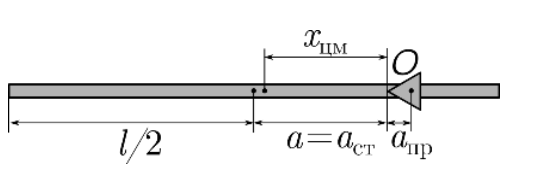
\includegraphics[scale=0.8]{pictures/рис 3.png}}
\caption{.\ \textit{Смещение центра масс из-за подвесной призмы}}
\end{figure}

\noindent
В итоге формула для периода примет вид:
\begin{equation}\label{eq11}
T = 2\pi \sqrt{\frac{\frac{l^2}{12} + a^2}{g (1+\frac{m_{\text{пр}}}{m_{\text{ст}}})x_{\text{ц}}}}
\end{equation}

\section*{\textbf{2. Ход работы.}}

\begin{itemize}
\item[\textbf{1}.] Заметим, что погрешности измерения $l$ и $a$ равны цене деления линейки, то есть \(\sigma_l = \sigma_a = 0.1 \text{ см.} \) Ускорение свободного падения можно найти, зная период, из формулы \eqref{eq3}:
\begin{equation}
g = \frac{4\pi^2}{T^2} l_{\text{пр}}
\end{equation}
\begin{flalign*} \text{Тогда } \varepsilon_g = \sqrt{(2\varepsilon_T)^2+(\varepsilon_{l_{\text{пр}}})^2}. \text{ Обозначим } f(l, a) \equiv l_{\text{пр}} \equiv \frac{l^2}{12a} + a \text{. Тогда:}&& \end{flalign*}

\[ \frac{\partial{f}}{\partial{l}} = \frac{l}{6a} \quad ; \quad \frac{\partial{f}}{\partial{a}} = 1 - \frac{l^2}{12a^2}   \]

\[\varepsilon_f = \frac 1 f \sqrt{\left(\frac{\partial{f}}{\partial{l}}\sigma_l\right)^2 + \left(\frac{\partial{f}}{\partial{a}}\sigma_a\right)^2} = \frac{\sigma_a}{\frac{l^2}{12} + a^2} \sqrt{\frac{l^2}{36a^2} + \left(1-\frac{l^2}{12a^2} \right)^2  }\]

\noindent
\begin{flalign}\label{eq13} \text{Пусть } \mu = l/a \text{. Тогда получим: } \varepsilon_f =  \frac{12}{13\mu} \sqrt{\frac{\mu^2}{36} + \left(1-\frac{\mu^2}{12}\right)^2}\frac{\sigma_a}{l} \ .&& \end{flalign} Построим график функции $\varepsilon_f(\mu)$ для $\mu \in [2; 10]$ и $l = 1 \text{ м}$ (примерно в таком диапазоне мы будем производить измерения). График показан на Рис. 4. Нетрудно видеть, что ошибка измерения $l_{\text{пр}}$ на всём диапазоне не превосходит $0.1 \%$. Примерно с такой точностью есть смысл измерять период $T$.
\begin{figure}[h]
\center{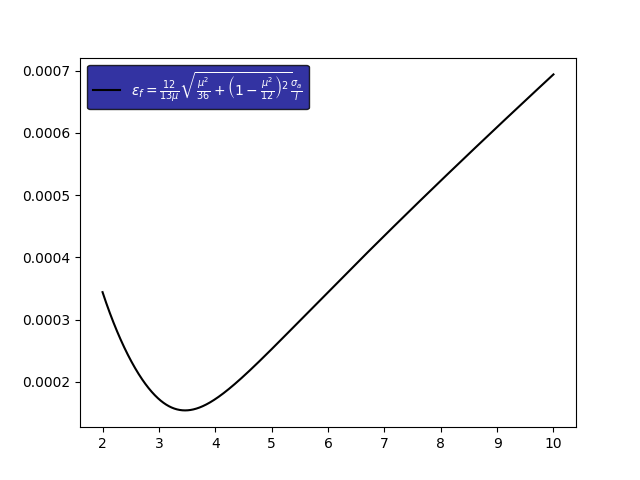
\includegraphics[scale=0.8]{pictures/Figure_1.png}}
\caption{.\ \textit{График зависимости} $\varepsilon_f(\mu)$ \textit{для} $\mu \in [2; 10]$}
\end{figure}
\item[\textbf{2}.] Измерим длину $l$ стержня линейкой, взвесим стержень и призму на электронных весах, определим расстояние от края пустого стержня до его центра масс. Получим (погрешность измерения массы на весах оценили как единицу последнего разряда, т. е. $\sigma_m = 0.1$  г):
\[l = (100  \pm  0.1) \text{ см} \ ; \ m_{\text{пр}} = (74.9  \pm  0.1) \text{ г} \ ; \ m_{\text{ст}} = (1022.4  \pm  0.1) \text{ г}\]
\[ X_{\text{ц}} = (50.0  \pm  0.1) \text{ см}  \]

Нетрудно видеть, что расстояние от края стержня до его центра масс $X_{\text{ц}} = l/2$, поэтому будем измерять $a$ от оси до середины стержня. Расстояние $x_{\text{ц}}$ от центра масс стержня с призмой до оси будем вычислять по формуле:
\begin{equation}
x_{\text{ц}} = a - (X_{\text{ц}} - x^{'}_{\text{ц}}),
\end{equation}
где $x^{'}_{\text{ц}}$ - расстояние от края стержня до центра масс.
\item[\textbf{3}.] Установим призму на некотором расстоянии от середины стержня, и измерим $a$ и $x^{'}_{\text{ц}}$. Получим:
\[a = (45.0  \pm  0.1) \text{ см} \ ; \ x^{'}_{\text{ц}} = (46.8  \pm  0.1) \text{ см} \ ; \ x_{\text{ц}} = (41.8  \pm  0.2) \text{ см}\]
Погрешность измерения $x_{\text{ц}}$ считалась, как:
\begin{equation}
\sigma_{x_{\text{ц}}} = \sqrt{\sigma_a^2 + \sigma_{X_{\text{ц}}}^2 + \sigma_{{x^{'}_{\text{ц}}}}^2} =  \sigma_a \sqrt{3} \approx 0.2 \text{ см}
\end{equation}
\item[\textbf{4}.] Проведём предварительный опыт. Устанавливаем маятник на консоли, отклоняем на малый угол (не более $5^{\circ}$) , убеждаемся, что он качается без помех, призма не просклальзывает, колебания затухают слабо. Измеряем время $n=20$ полных колебаний маятника и вычисляем период $T$ \[t_{20} = (31.91  \pm  0.01) \text{ с} \quad ; \quad T = \frac{t_{20}}{n} \approx (1.5955 \pm 0.0005) \text{ с}\]
Здесь за систематическую погрешность измерения времени секундомером была принята единица последнего разряда $\sigma_t = 0.1 \text{ с}$, а $\sigma_T = \sigma_{t_{20}}/n = 0.0005 \text{ с}$

\noindent
Вычислим предварительное значение $g$ по формуле \eqref{eq3}:
\begin{equation}
g = \frac{4\pi^2}{T^2} \left(\frac{l^2}{12a} + a\right) \approx (9.850 \pm 0.007) \ \frac{\text{м}}{\text{с}^2}
\end{equation}

\noindent
Здесь погрешность $g$ считалась по формулам, приведённым в пункте 1, в частности $\varepsilon_f$ считалось по формуле (\ref{eq13}) для $\mu = l/a = 20/9$, а $\varepsilon_T = \varepsilon_{t_{20}}$. Получили отклонение от теоретического значения $g$ не более $10\%$.

\item[\textbf{5}.] Проведём серию из $N = 10$ измерений времени $t_{20}$ полных $n = 20$ колебаний стержня. Результаты - в табл. 1.
% \usepackage{booktabs}


\begin{table}[h]
\centering
\begin{tabular}{|c|c|} 
\hline
$N$ опыта & $t_{20}$, с \\ 
\hline
1           & 31.91             \\ 
\hline
2           & 31.90             \\ 
\hline
3           & 32.07             \\ 
\hline
4           & 31.87             \\ 
\hline
5           & 31.84             \\ 
\hline
6           & 31.94             \\ 
\hline
7           & 31.82             \\ 
\hline
8           & 31.90             \\ 
\hline
9           & 32.00             \\ 
\hline
10          & 31.98             \\
\hline

\end{tabular}
\caption{}
\end{table}

Вычислим среднее значение и ошибки измерения времени $t_{20}$:
\begin{equation}
t_{20} = \overline{t_{20}} = \frac{\sum\limits_{i=1}^N t_{20, i}}{N} = (31.92 \pm 0.07) \text{ с} \ ; \ \sigma_{t_{20}}^{\text{случ}} = \sqrt{\frac{\sum\limits_{i=1}^N (t_{20, i} - t_{20})^2}{N(N-1)}} \approx 0.07 \text{ с}
\end{equation}
\begin{equation}
\sigma_{t_{20}}^{\text{сист}} = 0.01 \text{ с} \quad ; \quad \sigma_{t_{20}}^{\text{полн}} = \sqrt{\sigma_{t_{20}}^{\text{случ}^2} + \sigma_{t_{20}}^{\text{сист}^2}} \approx 0.07 \text{ с} \quad ; \quad \varepsilon_{t_{20}} \approx 2 \cdot 10^{-3} 
\end{equation}
Для периода имеем: $T = (1.596 \pm 0.004) \text{ с}$. Заметим, что точность измерения $T$ порядка $0.1\%$, поэтому изменять $n$ не будем. Значение $g$ определим по более точной формуле \eqref{eq11}:
\begin{equation}
g = \frac{4\pi^2}{T^2} \frac{\frac{l^2}{12} + a^2}{\left(1+\frac{m_{\text{пр}}}{m_{\text{ст}}}\right) x_{\text{ц}}}
\end{equation}
Заметим, что знаменатель второй дроби близок к $a$, $\sigma_{x_{\text{ц}}} = \sigma_a \sqrt{3}$, а относительная  погрешность определения $\psi = (1 + m_{\text{пр}}/m_{\text{ст}})$:
\[\varepsilon = \frac{\sigma_{\frac{m_{\text{пр}}}{m_{\text{ст}}}}}{\psi} \approx  \frac{\frac{\sigma_{m_{\text{пр}}}}{m_{\text{ст}}}}{\psi} \approx 10^{-4} \]
Поэтому будем считать $\sigma_g$ по формулам из п.1 аналогично тому, как делали при предварительном расчёте. Получим:
\[ g = (9.87 \pm 0.04) \ \frac{\text{м}}{\text{с}^2} \]

\item[\textbf{6}.] Проведём аналогичные измерения ещё для $9$ значений $a$. При этом вблизи минимума периода $a_m = \frac{l}{2\sqrt{3}}$ стоит провести больше измерений. Результаты - в табл. 2-11.

\begin{table}
\begin{minipage}{0.32\linewidth}
\centering
\begin{tabular}{|l|l|}
\hline
\multicolumn{2}{|c|}{$a = 400 \text{ мм}$} \\
\hline
N опыта & $t_{20}$, с  \\
\hline
1       & 31.20             \\
\hline
2       & 31.24             \\
\hline
3       & 31.17             \\
\hline
4       & 31.38             \\
\hline
5       & 31.18             \\
\hline
6       & 31.09             \\
\hline
7       & 31.25             \\
\hline
8       & 31.25             \\
\hline
9       & 31.47             \\
\hline
10      & 31.12     \\
\hline       
\end{tabular}
\caption{}
\end{minipage}
\begin{minipage}{0.32\linewidth}
\centering
\begin{tabular}{|l|l|}
\hline
\multicolumn{2}{|c|}{$a = 350 \text{ мм}$} \\
\hline
N опыта & $t_{20}$, с  \\
\hline
1       &   30.78          \\
\hline
2       &   30.80             \\
\hline
3       &   30.71            \\
\hline
4       &   30.60            \\
\hline
5       &   30.72           \\
\hline
6       &   30.79             \\
\hline
7       &   30.75           \\
\hline
8       &   30.78             \\
\hline
9       &   30.72             \\
\hline
10      &   30.70    \\
\hline       
\end{tabular}
\caption{}
\end{minipage}
\begin{minipage}{0.32\linewidth}
\centering
\begin{tabular}{|l|l|}
\hline
\multicolumn{2}{|c|}{$a = 300 \text{ мм}$} \\
\hline
N опыта & $t_{20}$, с  \\
\hline
1       &   30.50          \\
\hline
2       &   30.53             \\
\hline
3       &   30.53            \\
\hline
4       &   30.47           \\
\hline
5       &   30.44           \\
\hline
6       &   30.44            \\
\hline
7       &   30.53           \\
\hline
8       &   30.53             \\
\hline
9       &   30.44             \\
\hline
10      &   30.66    \\
\hline       
\end{tabular}
\caption{}
\end{minipage}
\end{table}

\begin{table}
\begin{minipage}{0.32\linewidth}
\centering
\begin{tabular}{|l|l|}
\hline
\multicolumn{2}{|c|}{$a = 290 \text{ мм}$} \\
\hline
N опыта & $t_{20}$, с  \\
\hline
1       & 30.44             \\
\hline
2       & 30.28             \\
\hline
3       & 30.32           \\
\hline
4       & 30.44             \\
\hline
5       & 30.50             \\
\hline
6       & 30.38             \\
\hline
7       & 30.41            \\
\hline
8       & 30.43             \\
\hline
9       & 30.41             \\
\hline
10      & 30.37     \\
\hline       
\end{tabular}
\caption{}
\end{minipage}
\begin{minipage}{0.32\linewidth}
\centering
\begin{tabular}{|l|l|}
\hline
\multicolumn{2}{|c|}{$a = 280 \text{ мм}$} \\
\hline
N опыта & $t_{20}$, с  \\
\hline
1       &   30.37          \\
\hline
2       &   30.59             \\
\hline
3       &   30.25            \\
\hline
4       &   30.47            \\
\hline
5       &   30.50           \\
\hline
6       &   30.47             \\
\hline
7       &   30.41           \\
\hline
8       &   30.47             \\
\hline
9       &   30.62             \\
\hline
10      &   30.40    \\
\hline       
\end{tabular}
\caption{}
\end{minipage}
\begin{minipage}{0.32\linewidth}
\centering
\begin{tabular}{|l|l|}
\hline
\multicolumn{2}{|c|}{$a = 270 \text{ мм}$} \\
\hline
N опыта & $t_{20}$, с  \\
\hline
1       &   30.65          \\
\hline
2       &   30.40             \\
\hline
3       &   30.53            \\
\hline
4       &   30.72          \\
\hline
5       &   30.87           \\
\hline
6       &   30.50            \\
\hline
7       &   30.70          \\
\hline
8       &   30.84             \\
\hline
9       &   30.40             \\
\hline
10      &   30.44    \\
\hline       
\end{tabular}
\caption{}
\end{minipage}
\end{table}

\begin{table}
\begin{minipage}{0.32\linewidth}
\centering
\begin{tabular}{|l|l|}
\hline
\multicolumn{2}{|c|}{$a = 250 \text{ мм}$} \\
\hline
N опыта & $t_{20}$, с  \\
\hline
1       & 30.72             \\
\hline
2       & 30.62             \\
\hline
3       & 30.60           \\
\hline
4       & 30.72             \\
\hline
5       & 30.78             \\
\hline
6       & 30.69             \\
\hline
7       & 30.81           \\
\hline
8       & 30.41           \\
\hline
9       & 30.59            \\
\hline
10      & 30.56     \\
\hline       
\end{tabular}
\caption{}
\end{minipage}
\begin{minipage}{0.32\linewidth}
\centering
\begin{tabular}{|l|l|}
\hline
\multicolumn{2}{|c|}{$a = 208 \text{ мм}$} \\
\hline
N опыта & $t_{20}$, с  \\
\hline
1       &   31.25          \\
\hline
2       &   31.31             \\
\hline
3       &   31.25           \\
\hline
4       &   31.34            \\
\hline
5       &   31.32           \\
\hline
6       &   31.28             \\
\hline
7       &   31.35         \\
\hline
8       &   31.31             \\
\hline
9       &   31.26             \\
\hline
10      &   31.28    \\
\hline       
\end{tabular}
\caption{}
\end{minipage}
\begin{minipage}{0.32\linewidth}
\centering
\begin{tabular}{|l|l|}
\hline
\multicolumn{2}{|c|}{$a = 150 \text{ мм}$} \\
\hline
N опыта & $t_{20}$, с  \\
\hline
1       &   33.66          \\
\hline
2       &   33.79             \\
\hline
3       &   33.69            \\
\hline
4       &   33.60          \\
\hline
5       &   33.75           \\
\hline
6       &   33.72            \\
\hline
7       &   33.65          \\
\hline
8       &   33.75             \\
\hline
9       &   33.66             \\
\hline
10      &   33.70    \\
\hline       
\end{tabular}
\caption{}
\end{minipage}
\end{table}

\begin{table}[]
\begin{tabular}{|l|l|l|l|l|l|l|l|}
\hline
\textnumero \  серии & $a$, мм      & $x^{'}_{\text{ц}}$, мм & $x_{\text{ц}}$, мм & $n$ & $t_{20}$, с      & $T$, с            & $g$, $\text{м}/\text{с}^2$ \\ \hline
1        & $450 \pm 1 $ & $468 \pm 1$            & $418 \pm 2$        & 20  & $31.92 \pm 0.07$ & $1.596 \pm 0.004$ & $9.87 \pm 0.04$            \\ \hline
2        & $400 \pm 1$  & $475 \pm 1$            & $375 \pm 2$        & 20  & $31.24 \pm 0.11$ & $1.562 \pm 0.006$ & $9.78 \pm 0.07$            \\ \hline
3        & $350 \pm 1$  & $476 \pm 1$            & $326 \pm 2$        & 20  & $30.74 \pm 0.06$ & $1.537 \pm 0.003$ & $9.83 \pm 0.04$            \\ \hline
4        & $300 \pm 1$  & $478 \pm 1$            & $278 \pm 2$        & 20  & $30.51 \pm 0.06$ & $1.526 \pm 0.003$ & $9.85 \pm 0.04$            \\ \hline
5        & $290 \pm 1$  & $479 \pm 1$            & $269 \pm 2$        & 20  & $30.40 \pm 0.06$ & $1.520 \pm 0.003$ & $9.91 \pm 0.04$            \\ \hline
6        & $280 \pm 1$  & $480 \pm 1$            & $260 \pm 2$        & 20  & $30.44 \pm 0.10$ & $1.522 \pm 0.005$ & $9.87 \pm 0.07$            \\ \hline
7        & $270 \pm 1$  & $481 \pm 1$            & $251 \pm 2$        & 20  & $30.61 \pm 0.17$ & $1.531 \pm 0.009$ & $9.77 \pm 0.11$            \\ \hline
8        & $250 \pm 1$  & $482 \pm 1$            & $232 \pm 2$        & 20  & $30.65 \pm 0.11$ & $1.533 \pm 0.006$ & $9.84 \pm 0.07$            \\ \hline
9        & $208 \pm 1$  & $485 \pm 1$            & $193 \pm 2$        & 20  & $31.30 \pm 0.03$ & $1.565 \pm 0.002$ & $9.85 \pm 0.02$            \\ \hline
10       & $150 \pm 1$  & $489 \pm 1$            & $139 \pm 2$        & 20  & $33.70 \pm 0.05$ & $1.685 \pm 0.003$ & $9.86 \pm 0.03$            \\ \hline
\end{tabular}
\caption{}
\end{table}
\item[\textbf{7}.] Для $a = 40$ см $l_{\text{пр}} \approx 60.8 $ см. Установим эту длину у математического маятника и проведём опыт из $K = 7$ измерений времени $t_{20}$ полных $n = 20$ колебаний маятника. Результат - в таблице 12.
\begin{table}[h!]
\centering
\begin{tabular}{|l|l|}
\hline
N опыта & $t_{20}$, с  \\
\hline
1       &   33.66          \\
\hline
2       &   33.79             \\
\hline
3       &   33.69            \\
\hline
4       &   33.60          \\
\hline
5       &   33.75           \\
\hline
6       &   33.72            \\
\hline
7       &   33.65          \\
\hline       
\end{tabular}
\caption{}
\end{table}
\begin{flalign*}\text{Отсюда получим: } t_{20} = (31.32 \pm 0.12) \text{ с} \ ; \ T_{math} = (1.566 \pm 0.006) \text{ с} && \end{flalign*}
Так как при этом $T_{phys} = (1.562 \pm 0.006) \text{ с}$ (табл. 11), то $\Delta T = T_{math} - T_{phys} = (0.004 \pm 0.008 )$ с, то есть в пределах погрешности значения $T_{math}$ и $T_{phys}$ \textit{совпадают}.


Заметим, что для $a_1 = 40$ см, $a_2 = l_{\text{пр}}(a_1) - a_1 \approx 20.8 $ см. Из таблицы 11:
\[T(a_1) = (1.562 \pm 0.006) \text{ с} \ ; \ T(a_2) = (1.565 \pm 0.002) \text{ с} \]
\[ \Delta T = T(a_2) - T(a_1) = (0.003 \pm 0.006) \text{с}\]
В пределах погрешности $T(a_1)$ и $T(a_2)$ совпадают, что подтверждает \textit{теорему Гюйгенса}.
\item[\textbf{8}.] По данным табл. 11 усредним $g$:
\[g =\frac{\sum\limits_{i=1}^{10} g_i}{10} =(9.843 \pm 0.019) \frac{\text{м}}{\text{с}^2} \ ; \ \varepsilon_g = 2 \cdot 10^{-3}\]
Погрешность $g$ считалась, как:
\[ \sigma_g = \frac{1}{10} \sqrt{\sum\limits_{i=1}^{10} \sigma^2_{g_i}}  \]

\item[\textbf{9}.] Построим экспериментальную зависимость $T(a)$ по данным табл. 11. Зависимость имеет минимум между $a = 28$ см и $a = 29$ см, что согласуется с теорией: $a_m = \frac{l}{2\sqrt{3}} \approx 28.87$ см. Построим также теоретическую кривую $T(a)$ при $a \in [14; 50]$ см. Она задаётся формулой: 
\begin{equation}
 T(a) = 2\pi \sqrt{\frac{\frac{l^2}{12} + a^2}{ga}} = 2\pi \sqrt{\frac{z^2+a^2}{ga}} = 2\pi \sqrt{\frac{z}{a}} \sqrt{\frac{z}{a}+\frac{a}{z}} \quad \left(z^2 = \frac{l^2}{12} \right) 
\end{equation}
Отсюда видно, что $T=T_m$ при $a = z$, при этом зависимость $T(a)$ можно переписать в виде:
\begin{equation}\label{eq21}
T(a) = \frac{T_m}{\sqrt{2}} \sqrt{\frac{z}{a}+\frac{a}{z}}
\end{equation}
Поэтому для проверки соответствия эксперимента теоретическим расчётам построим также график $T(a)$ по формуле \eqref{eq21} для экспериментального значения $T_m \approx 1.520$ с. Соответсвующие графики приведены на рис. 5, 6, 7.
\begin{figure}
\center{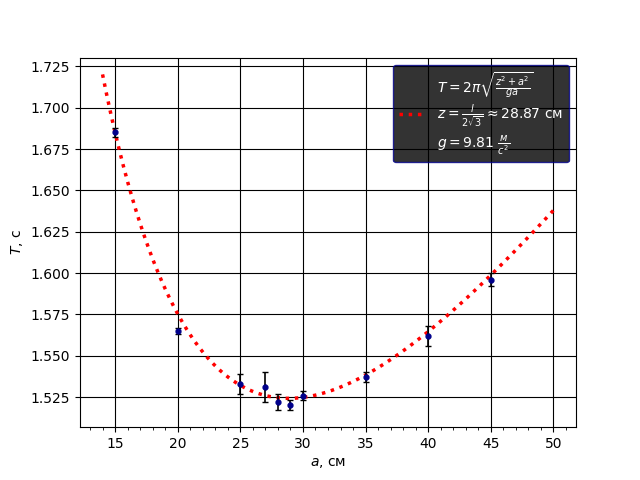
\includegraphics[scale=1]{pictures/Figure_2.png}}
\caption{. \textit{Экспериментальная и теоретическая зависимость} $T(a)$}
\end{figure}
\begin{figure}
\center{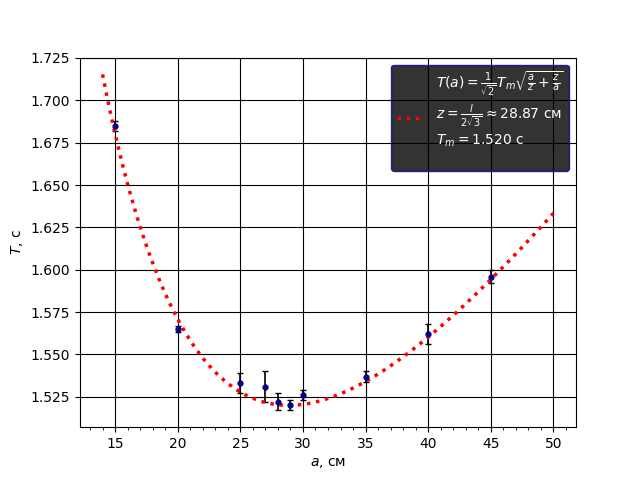
\includegraphics[scale=1]{pictures/Figure_3.png}}
\caption{. \textit{Экспериментальная и теоретическая зависимость} $T(a)$}
\end{figure}
\begin{figure}
\center{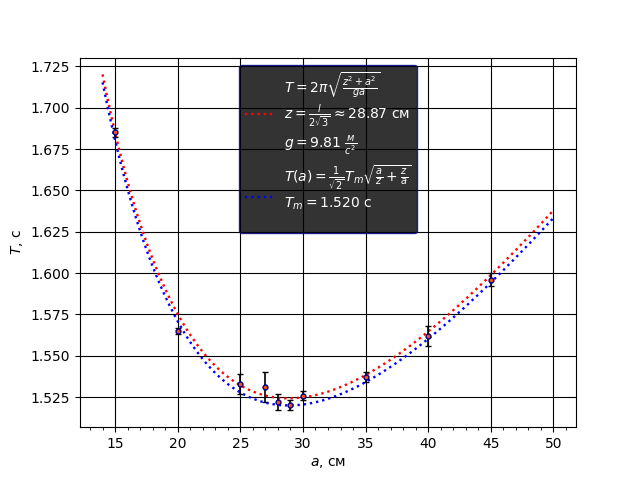
\includegraphics[scale=1]{pictures/Figure_4.png}}
\caption{. \textit{Экспериментальная и теоретические зависимости} $T(a)$ }
\end{figure}
Нетрудно видеть, что точки в пределах погрешности ложатся на теоретические кривые, а кривая, построенная с использованием экспериментального $T_m$, близка к теоретической кривой.
\item[\textbf{10}.] Построим график зависимости $u(v)$, где $u = T^2 x_{\text{ц}}$, v = $a^2$. При этом ошибки величин $u$ и $v$ будем считать по формулам:
\begin{equation}
\sigma_u = \sqrt{(T^2 \sigma_{x_{\text{ц}}})^2+(2 T \sigma_T x_{\text{ц}})^2} = T \sqrt{(T \sigma_{x_{\text{ц}}})^2+(2 x_{\text{ц}} \sigma_T)^2}
\end{equation}
\begin{equation}
\sigma_v = 2 a \sigma_a
\end{equation}
График зависимости и его аппроксимация линейной функцией по хи-квадрат показаны на рис. 8. 
\begin{figure}
\center{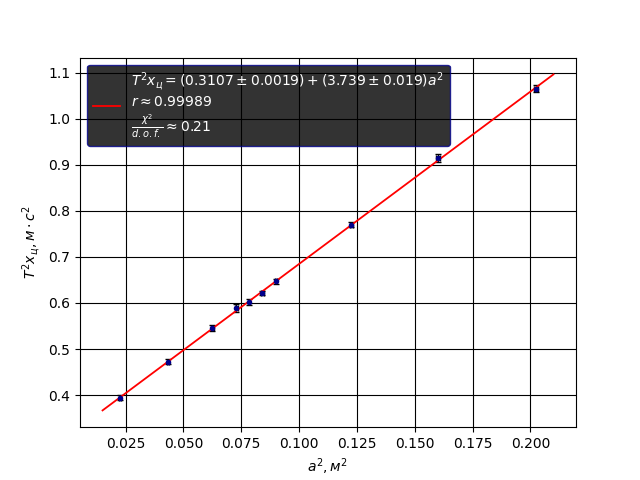
\includegraphics[scale=1]{pictures/Figure_5.png}}
\caption{. \textit{График зависимости} $u(v)$ \textit{и его аппроксимация линейной функцией} }
\end{figure}
Выразим коэффициенты зависимости $u(v)$ теоретически. Из формулы \eqref{eq11} получим:
\[T^2 x_{\text{ц}} = \frac{4\pi^2}{g \psi} a^2 + \frac{\pi^2 l^2}{3\psi g} \Rightarrow u = \frac{4\pi^2}{g\psi}v + \frac{\pi^2 l^2}{3\psi g} = \beta v + \alpha, \ \psi = \left(1 + \frac{m_{\text{пр}}}{m_{\text{ст}}}\right) \]
Обработка методом хи-квадрат даёт:
\[ \beta = (3.739 \pm 0.019) \frac{\text{с}^2}{\text{м}^2} \ ; \ \alpha =  (0.3107 \pm 0.0019) \text{м} \cdot \text{с}^2 \ ; \ r \approx 0.99989 \ (\textit{коэф. корреляции})\]
\[\frac{\chi^2}{d.o.f.} \approx 0.21 \]
В итоге получим: 
\[ g = \frac{4\pi^2}{\psi \beta} = (9.84 \pm 0.05) \frac{\text{м}}{\text{с}^2} \ ; \ \varepsilon_g = 5 \cdot 10^{-3}\]
Погрешность $g$, с учётом того, что $\varepsilon_{\psi} \ll \varepsilon_{\beta}$, считалась, как:
\[ \sigma_g = g \varepsilon_{\beta} = g \frac{\sigma_{\beta}}{\beta}  \]
\item[\textbf{11}.] Для $a = 40$ см измерим время $\tau_2$, за которое амплитуда колебаний маятника уменьшается в $2$ раза (c $10^{\circ}$ до $5^{\circ}$). Получим:
\[\tau_2 = (290.28 \pm 0.01) \text{ с}\]
\begin{flalign*}\text{Тогда время жизни: }\tau = \frac{\tau_2}{\ln{2}} \approx (418.78 \pm 0.01) \text{ с} \quad (\sigma_{\tau} = \tau \varepsilon_{\tau_2}) &&\end{flalign*}
\begin{flalign*}\text{Добротность: } Q = \pi \frac{\tau}{T(a)} \approx 842 \pm 8  \quad (\sigma_Q = Q \varepsilon_T). \text{ Система высокодобротна.}&&\end{flalign*}
\end{itemize}
\section*{\textbf{3. Вывод}}
\noindent
В ходе работы были проверены формулы для периода физического маятника и теорема Гюйгенса об обратимости точек опоры. Полученные экспериментальные данные хорошо согласуются с теоретическим описанием рассматриваемых явлений. Было исследовано затухание колебаний, найдено время жизни и добротность системы. Также было определено ускорение свободного падения $g$ двумя способами: путём усреднения значений, полученных в каждой серии измерений периода полных $n$ колебаний маятника и путём анализа экспериментальной зависимости периода колебаний от параметров установки. Точность измерений в обоих случаях примерно одинакова ($\sim 0.1 \%$), однако только второй способ дал значение, в пределах погрешности совпадающее с теоретическим $g = 9.81 \text{ м}/\text{с}^2$. Из этого можно сделать вывод, что анализ зависимостей, параметром которых является искомая величина, даёт более точные результаты, чем усреднение значений величины в каждой точке измерения. 
\end{document}